%! Author = jbf
%! Date = 31.07.25

\newpage
\section{Grundlagen}
\label{Grundlagen}
In diesem Kapitel werden die theoretischen Grundlagen für das Entwickeln der Software,
so wie das notwendige Verständnis des Testandes und seine Abläufe behandelt.
\subsection{Überblick über den Umrichter-Prüfstand}
In diesem Unterkapitel wird der Umrichter-Teststand, von dem die zu verarbeitenden Datensätze stammen beschrieben,
da dies für das generelle Verständnis der einzulernenden Datensatzstruktur unerlässlich ist.
Die genaue Bezeichnung des Teststandes „USTB DWT Test Bench (XCT0006-1)“ im weiteren als Test-Bench oder Teststand benannt.
Diese Art Teststand wird im allgemein für die End-of-Line Prüfung von unterschiedlichen Umrichtern nach ihrer Herstellung genutzt,
um die Produktqualität und -funktionalität sicherzustellen.\cite*{Main_Manuel_USTB2018}

In dem hier vorliegenden Fall wird der Teststand verwendet, um die aus dem Feld kommenden Umrichter auf ihre weiter Nutzungstauglichkeit zu testen.
Die weiter Nutzungstauglichkeit wird ermittelt, indem die Messwerte mit Mittelwerten, die von mehreren fabrikneuen Umrichtern stammenden verglichen werden.
Diese Messwerte müssen sich in einen vorher definierten Toleranzbereich befinden, um weiter verwenden zu werden.

Die Test-Bench besteht aus mehreren Hauptkomponenten:
\begin{itemize}
\item Das Netzteil, welches mit einer 400V Netzspannung versorgt wird, wandelt diese in eine Gleichspannung. Das Netzteil leifert maximal 8kW mit 1200VDC oder 800VDC, welche Werte verwendet werden kann vor Teststart bestimmt werden. In Abbildung 1\ref{fig:1. Aufbau des Teststandes} mit PSU bezeichnet, für „Power Supply Unit“.
\item Das Elektronik-Rack, auf dem Mess- und Control-Komponenten befestigt sind. Hier befinden sich auch der (XCS2100) System-Controller der das ganze System mit dem PC, auf dem die Test-Bench Software läuft, via Ethernet verbindet. In Abbildung \ref{fig:1. Aufbau des Teststandes} mit ER bezeichnet, für „Electronic Rack“.
\item Der Testmatrix-Schrank, in dem die Sammelschienen für den Stromanschluss und den Schützen sitzen. In Abbildung \ref{fig:1. Aufbau des Teststandes} mit TM bezeichnet, für „Test Matrix cabine“.
\item Der Schrank mit dem Kühlungssystem, da die Umrichter während des Betriebes Wassergekühlt werden müssen. In Abbildung \ref{fig:1. Aufbau des Teststandes} mit „Cool1“ bezeichnet.
\item Dem Carrier, auf dem Umrichter befestigt werden. Dieser wird speziell für bestimmte Umrichter konstruiert. In Abbildung \ref{fig:1. Aufbau des Teststandes} mit Carrier1 bezeichnet.

\end{itemize}


\begin{figure}[h]
    \centering
    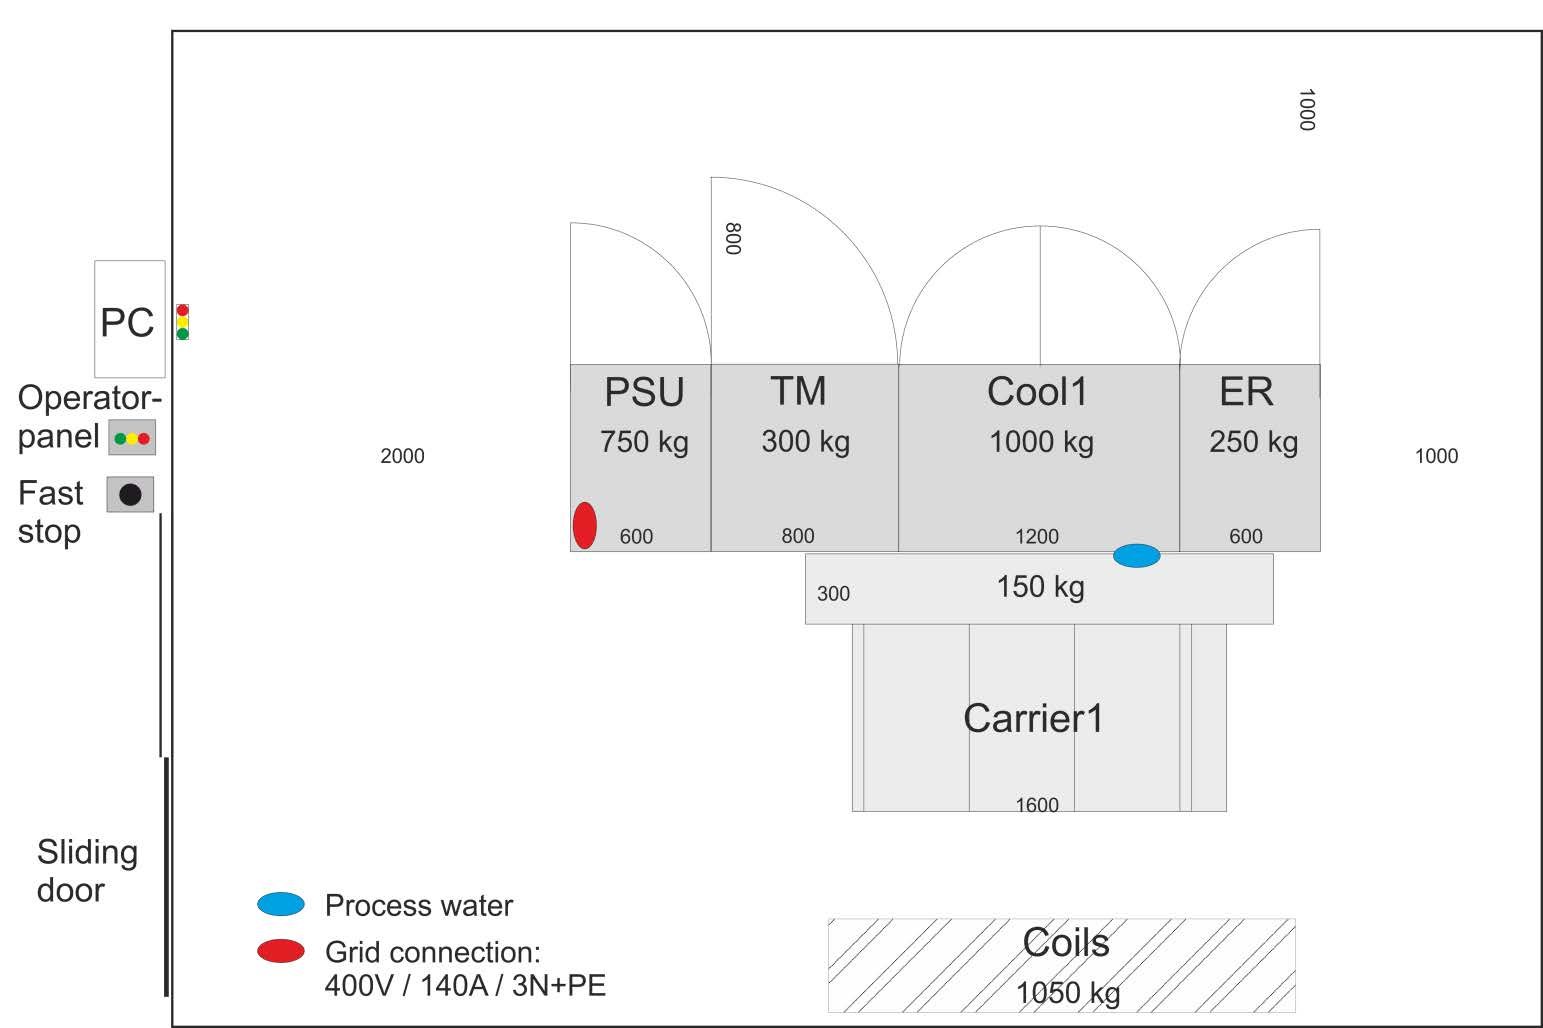
\includegraphics[width=0.8\textwidth]{Grafiken/Test Cabin.jpg}
    \caption{Aufbau des Teststandes}
    \label{fig:1. Aufbau des Teststandes}
    {Quelle: \cite*[7]{Main_Manuel_USTB2018}}
\end{figure}


Neben dem Hauptkomponenten befinden sich außerhalb des Sicherheitsbereiches, der während des Betriebes nicht betreten werden darf,
ein PC mit einer Software zum Steuern der Testeinrichtung, sowie eine Betriebsanzeige und ein Notaus. \cite*{Main_Manuel_USTB2018}

\newpage

Ein Test läuft wie folgt ab:

\begin{enumerate}
\item Die Umrichter werden auf dem Carrier befestigt, es werden meist 3 Umrichter gleichzeitig getastet, Abweichungen je nach Bauform der Umrichter.
Ab diesem Zeitpunkt werden die Umrichter in der gegebenen Fachliteratur als \ac{DUTs} bezeichnet, dies kommt auch in den Testberichten vor, daher hat der Autor diesen Begriff einzuführen und fortan zu übernehmen.


\item Durchführung des Driver Consumption Testes.


\item Durchführung des Pulse Testes.


\item Durchführung des Driver Power Testes.


\item Nach dem Durchlaufen eines Tests wird automatische ein XML-Datenfile mit den erhobenen Messdaten generiert, die enthalt die Messwerte und alle vorher bestimmten Einstellungen.


\end{enumerate}
Es gibt verschiedene Testmodule, die auf dem Teststand laufen.
Einige der verschiedenen Funktionen eines DUT können mit dem gleichen Modus eines Testmoduls überprüft werden, indem die entsprechenden Parametersätze ausgewählt werden.
Jeder Test ist autonom und kann mehrmals ausgeführt werden, auch mit unterschiedlichen Parametersätzen.
\\
Im Folgenden wird eine kurze Beschreibung der Funktionen der für diese Arbeit relevanten Testmoduls gegeben.

Driver Consumption Test:

Der Driver-Stromverbrauchstest überprüft den Stromverbrauch des Treibers im Leerlauf und während der PWM-Schaltung.

Pulse Test:

Der Impulstest verfügt über drei Funktionsmodi.
\begin{itemize}
    \item Im Modus „Funktionsschaltung“ (FSW) kann überprüft werden, ob die Halbleiter generell schalten.
    \item Im Modus „Überstromschutz“ (OCP) kann die Überstromüberwachung („weicher Kurzschluss“) überprüft werden.
    \item Im Modus „Dynamischer Kurzschlussschutz“ (DSCP) wird das korrekte Verhalten der Treiberstufe in Bezug auf einen harten Kurzschluss überprüft.
\end{itemize}

Power Test:

Mit diesem Test können zwei verschiedene Funktionen getestet werden:
\begin{itemize}
    \item Einerseits eignet sich der Burn-In-Test (BIT) dazu, die DUTs zyklisch zu betreiben und so reale Betriebszustände zu simulieren.
    \item Andererseits kann durch Überprüfung der Kühltemperatur am Ende des Tests die korrekte Wärmeübertragung der Halbleiter überprüft werden.
\end{itemize}
\\
Während des Übertemperaturschutz-Tests (OTP) wird ein DUT mit reduzierter Kühlung betrieben, bis die maximal zulässige
Kühlkörpertemperatur erreicht ist und die Temperaturschutzschaltung auslöst.


\subsection{Verarbeitung von XML-Daten}

XML, die Abkürzung für Extensible Markup Language, ist eine der beliebtesten Auszeichnungssprachen, die entwickelt wurde,
um Informationen in einem maschinenlesbaren und strukturierten Format zu speichern und zu transportieren.
Es ist eine textbasierte Auszeichnungssprache, die heute in vielen Anwendungen verwendet wird, wie z.B. Webdiensten,
Datenbanken, Konfigurationsdateien und vielen anderen.
XML ermöglicht die hierarchische Organisation von Informationen in einer strukturierten Weise, die sowohl für Menschen
als auch für Maschinen verständlich ist.

Die Motivation hinter XML war, eine universelle und erweiterbare Sprache zu schaffen, die von verschiedenen Systemen
unabhängig von der zugrunde liegenden Technologie genutzt werden kann.
Die Fähigkeit, Daten in einem offenen Standard zu speichern und auszutauschen, war entscheidend,
um die Interoperabilität zwischen verschiedenen Anwendungen und Plattformen zu fördern.

\subsubsection{XML-Strukturaufbau}

Ein XML-Dokument besteht aus einer Reihe von Elementen, die durch Tags markiert sind.
Die grundlegenden Bestandteile eines XML-Dokuments sind:

Prolog: Ein optionaler Abschnitt, der die XML-Version und die verwendete Zeichencodierung definiert.
Ein typischer Prolog sieht so aus:

\begin{figure}[H]
\centering
\begin{minipage}{0.95\textwidth}
\begin{lstlisting}[language=XML]
<?xml version="1.0" encoding="UTF-8"?>
\end{lstlisting}
\end{minipage}
\caption{XML Prolog Beispielcode}
\label{fig:XML Prolog Beispielcode}
    {Quelle: eigene Darstellung}
\end{figure}

Elemente: Die eigentlichen Daten werden in Elementen gespeichert, die mit einem Start-Tag beginnen und mit einem End-Tag abschließen.
Ein Element kann weitere Elemente enthalten, was zu einer hierarchischen Struktur führt:

\begin{figure}[H]
\centering
\begin{minipage}{0.95\textwidth}
\begin{lstlisting}[language=XML]
<buch>
  <titel>XML-Grundlagen</titel>
  <autor>Max Mustermann</autor>
</buch>
\end{lstlisting}
\end{minipage}
\caption{XML Elemente Beispielcode}
\label{fig:XML Elemente Beispielcode}
    {Quelle: eigene Darstellung}
\end{figure}

Attribute: Jedes Element kann Attribute haben, die zusätzliche Informationen enthalten.
Attribute werden im Start-Tag eines Elements definiert:

\begin{figure}[H]
\centering
\begin{minipage}{0.95\textwidth}
\begin{lstlisting}[language=XML]
<buch genre="Lehrbuch">
  <titel>XML-Grundlagen</titel>
  <autor>Max Mustermann</autor>
</buch>
\end{lstlisting}
\end{minipage}
\caption{XML Attribute Beispielcode}
\label{fig:XML Attribute Beispielcode}
    {Quelle: eigene Darstellung}
\end{figure}

Kommentare: Kommentare werden mit den Tags <!-- und --> eingefügt und dienen der Dokumentation oder dem Hinweis auf bestimmte Teile des Codes,
Sie werden beim Parsen des Dokuments ignoriert. In Abbildung \ref{fig:XML Kommentare Beispielcode} ist ein Beispiel wie
ein Kommentar genutzt wird.

\begin{figure}[H]
\centering
\begin{minipage}{0.95\textwidth}
\begin{lstlisting}[language=XML]
<!-- Dies ist ein Kommentar -->
\end{lstlisting}
\end{minipage}
\caption{XML Kommentare Beispielcode}
\label{fig:XML Kommentare Beispielcode}
    {Quelle: eigene Darstellung}
\end{figure}

Textinhalt: Zwischen den Start- und End-Tags eines Elements kann Text enthalten sein:

\begin{figure}[H]
\centering
\begin{minipage}{0.95\textwidth}
\begin{lstlisting}[language=XML]
<titel>XML-Grundlagen</titel>
\end{lstlisting}
\end{minipage}
\caption{XML Text Beispielcode}
\label{fig:XML Text Beispielcode}
    {Quelle: eigene Darstellung}
\end{figure}

\subsubsection{Verarbeiten von XML-Dateien mit Python}

\pagebreak
\subsection{Datenbankentwurf und Normalisierung}

\subsection{Grundlagen der Datenvisualisierung}

\subsection{Anforderungen an modulare Softwareentwicklung}